\documentclass[10pt]{scrartcl}
\usepackage[latin1]{inputenc}
\usepackage{ngerman}
\usepackage{graphicx}
\newtheorem{Def}{Definition}
\newtheorem{Bem}[Def]{Bemerkung}
\newtheorem{Bsp}[Def]{Beispiel}
\author{Wolfgang Keller}
\title{Aufgabe des Monats M�rz}
\begin{document}
\maketitle
\section{Hintergrund}
In einem Land mit $n>0$ St�dten gibt es nur Einbahnstra�en. Je zwei (ungleiche) St�dte sind durch genau eine Stra�e verbunden.

\section{Aufgabe}
Man zeige, dass es eine Stadt (die wir "`Zentralstadt"' nennen wollen) gibt, von der jede andere Stadt entweder direkt oder �ber h�chstens eine Zwischenstadt erreichbar ist.

\begin{Bem}
Unter "`B ist von A direkt erreichbar"' wollen wir verstehen, dass es eine Einbahnstra�e von A nach B gibt und unter "`B ist von A �ber h�chstens eine Zwischenstadt erreichbar"' wollen wir verstehen, dass es eine von A und B unterschiedliche Stadt C gibt, so dass es Einbahnstra�en von A nach C und C nach B gibt.
\end{Bem}

\begin{Bsp}
Wir haben n=4 St�dte (Magdeburg, Halle, Dresden und Berlin), welche gem�� der Landkarte aus Abbildung \ref{fig:karte} mit Einbahnstra�en verbunden sind.

\begin{figure}[htbp]
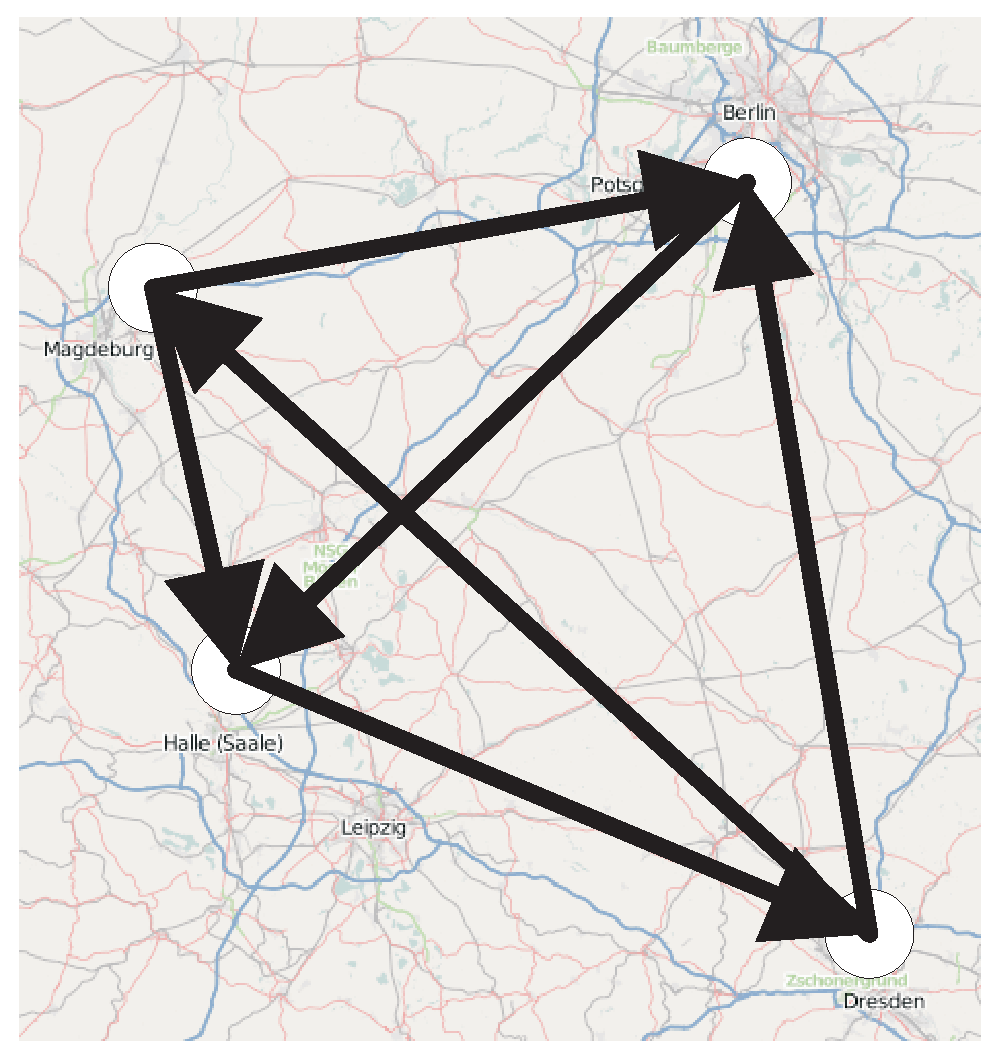
\includegraphics[width=0.5\textwidth]{karte}
\caption{Das Einbahnstra�ennetz aus dem Beispiel (Bildquelle: OpenStreetMap)}
\label{fig:karte}
\end{figure}

Dann sind in diesem Beispiel Magdeburg (da Berlin und Halle direkt und Dresden �ber Halle erreicht werden kann), Halle (da Dresden direkt und Berlin und Magdeburg �ber Dresden erreichbar sind) und Dresden (da Magdeburg und Berlin direkt und Halle �ber Magdeburg erreichbar sind) Zentralst�dte. Berlin ist keine Zentralstadt, da Magdeburg von Berlin weder direkt, noch �ber eine Zwischenstadt (sogar gar nicht) erreichbar ist.
\end{Bsp}

\section{Tipp}
Man versuche die zu beweisende Aussage mit dem Prinzip der "`vollst�ndigen Induktion"' zu zeigen, das hei�t: man zeigt
\begin{enumerate}
	\item die zu beweisende Aussage gilt alle Zahlen $\leq k$ an St�dten (beispielsweise k�nnten 1, 2 oder 3 in dieser Aufgabe sinnvolle Werte f�r k sein): dies bezeichnet man als "`Induktionsanfang"'
	\item wenn die Aussage f�r ein $m$ St�dte gilt (wobei $m\geq k$, aber ansonsten wissen wir nichts �ber m), so gilt sie auch f�r $m+1$: dies bezeichnet man als "`Induktionsschritt"'
\end{enumerate}
Durch das Induktionsaxiom der nat�rlichen Zahlen (nach Peano) wird gesichert, dass mittels dieses Beweisverfahrens die Aussage tats�chlich f�r alle nat�rlichen Zahlen n gilt (wenn du dich f�r weitere Details dar�ber interessierst, wende dich an deinen AG-Leiter).

Vorstellen kann man sich dieses Beweisverfahren als eine Art unendliche Dominoreihe, siehe dazu Abbildung \ref{fig:domino}.

\begin{figure}[htbp]
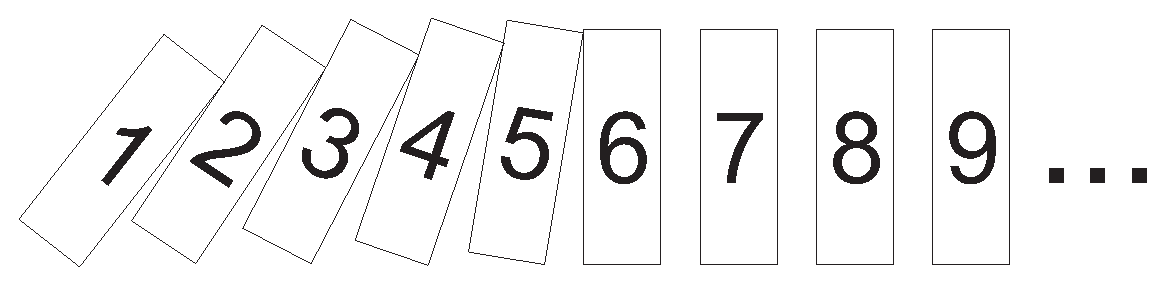
\includegraphics[width=0.7\textwidth]{domino}
\caption{Veranschaulichung des Prinzips der vollst�ndigen Induktion}
\label{fig:domino}
\end{figure}

Der Induktionsanfang sichert, dass die ersten k Dominosteine fallen werden und der Induktionsschritt, dass wenn ein Dominostein gefallen ist, auch der folgende f�llt. Somit fallen "`intuitiv"' alle Dominosteine. Mathematisch pr�zisiert wird diese Aussage durch das oben bereits genannte Induktionsaxiom der nat�rlichen Zahlen.
\end{document}